\subsection*{Level 1}
\addcontentsline{toc}{subsection}{Level 1}


Transforming the temporal criteria of the controller specification to frequency criteria leads to :
\begin{itemize}
 \item Cutoff frequency: $w_c t_r \approx 3 \Leftrightarrow w_c \approx 42.8 \text{ rad/s}$
 \item Phase margin: $D\% \leq 2\% \Leftrightarrow \Delta \Phi \geq 70^{\circ}$ (see Figure \ref{overshootMargin} for this criteria)
\end{itemize}

Moreover, since the position loop include a integrator, the steady state error will be zero.

\begin{center}
\begin{figure}[ht]
 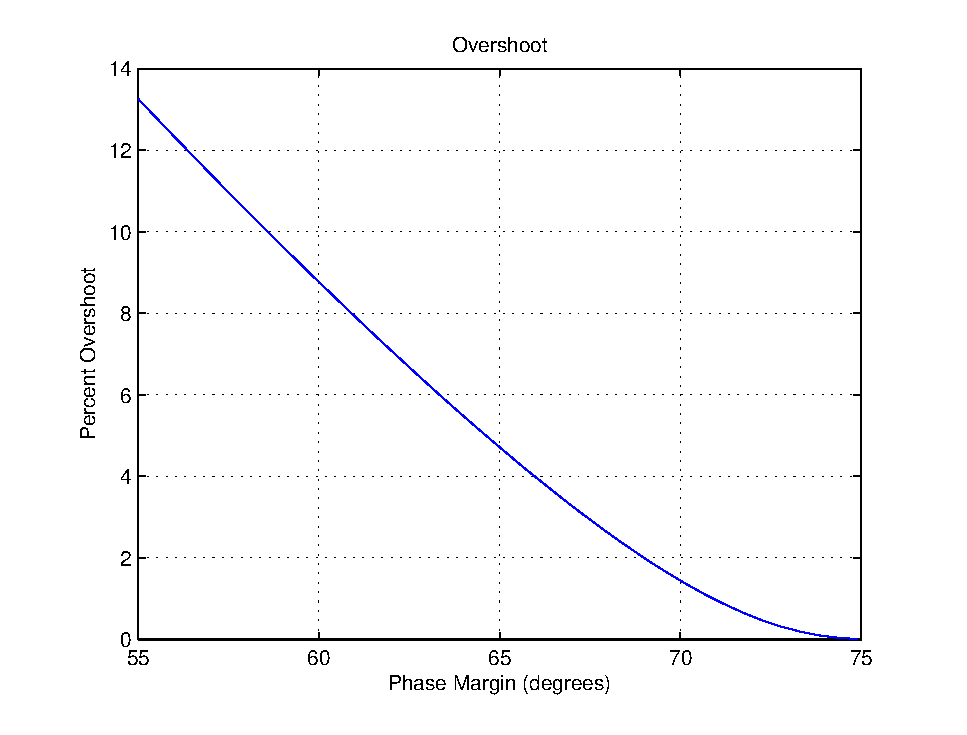
\includegraphics[width=\linewidth]{fig/overshootMargin.eps}
 \caption{Overshoot as a function of the phase margin}
 \label{overshootMargin}
\end{figure}
\end{center}

In this subsection, any sampling period can be used. Here, $T_s = 1 \text{ ms}$.

With the PI-controller from section \ref{velocont}, the ``continuous'' close loop transfer function of the system is:

\begin{equation}
 H_{cl,vel} = \frac{1}{1 + \frac{\tau_m}{K K_m}p}
\end{equation}

Therefore, outputting the position leads to the addition of an integrator block (integration of the velocity). The new transfer function is:

\begin{equation}
 H_{cl,pos} = \frac{1}{p}\frac{1}{1 + \frac{\tau_m}{K K_m}p}
\end{equation}

The maximum rise time for the velocity controller verify $t_{r,vel} \leq 5O \text{ ms} \Leftrightarrow w_c = 125.6 \text{ rad/s}$. Therefore, in the worst case scenario, the transfer function for the position is:

\begin{equation}
 H_{cl,pos} = \frac{1}{p} \frac{1}{1 + \frac{p}{125.6}}
\end{equation}

Figure \ref{bodePos} shows the bode diagram of this function.

\begin{center}
\begin{figure}[ht]
 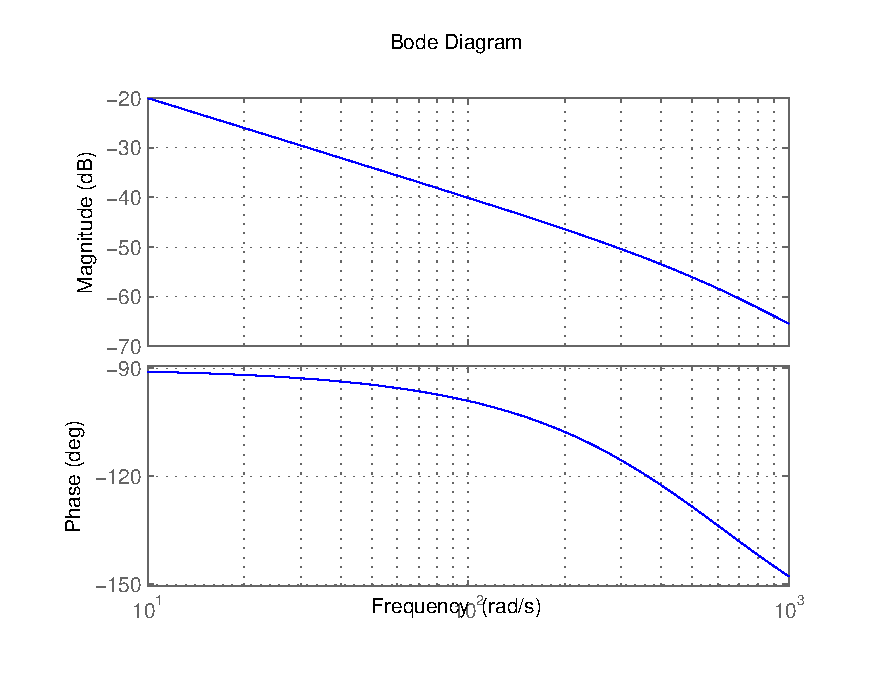
\includegraphics[width=\linewidth]{fig/bodePos.eps}
 \caption{Bode diagram of $H_{cl,pos}$}
 \label{bodePos}
\end{figure}
\end{center}

According to the bode diagram on Figure \ref{bodePos}, we have:

\begin{itemize}
 \item $G_{dB,pos}(\omega = 42.8 \text{ rad/s}) = -32 \text{ dB}$
 \item $\Delta \Phi = 86.3^{\circ}$
\end{itemize}

Therefore, we only need to translate vertically the gain curves in order to fulfill the criteria.

\emph{We use a proportional controller.}

Therefore:

$$ G_{dB,cont}(\omega = 42.8 \text{ rad/s}) = 32 \text{ dB} \Leftrightarrow K_P = 10^{\frac{32}{20}} = 40$$

Figure \ref{StepPPos} shows the step response of the system. \emph{All of the criteria are met.}

\begin{center}
\begin{figure}[ht]
 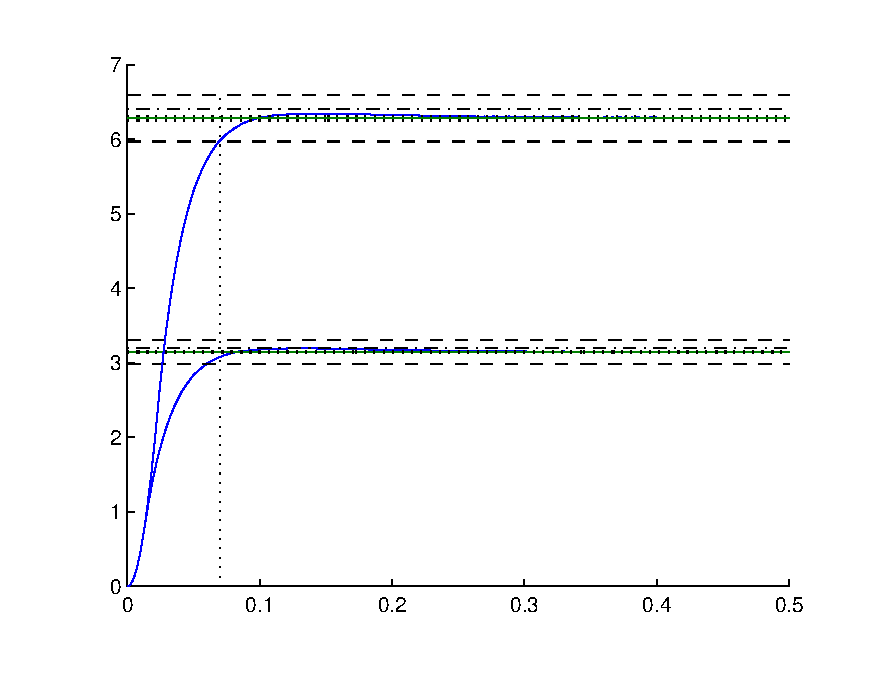
\includegraphics[width=\linewidth]{fig/StepPPos.eps}
 \caption{Steps responses of the system controled in position for two differents amplitudes}
 \label{StepPPos}
\end{figure}
\end{center}

\subsection*{Level 2}
\addcontentsline{toc}{subsection}{Level 2}
%---------------------------------------------
% WARNING: Missing subsection
%---------------------------------------------

Bla bla...






